\section{Choice of BLAS Library}
\label{subseq:blas-comparison}


To perform columns elimination of fully summed block of frontal matrices, MUMPS intensively uses GEMM, TRSM and GETRF subroutines which are parts of BLAS and LAPACK libraries. As an example, figure \ref{fig:mumps:steps-of-type-2-factorization} demonstrates factorization of a type 2 node.\\


\figpointer{\ref{fig:mumps:type-2-frontal-matrix}}
\begin{figure}[htpb]
  \centering
  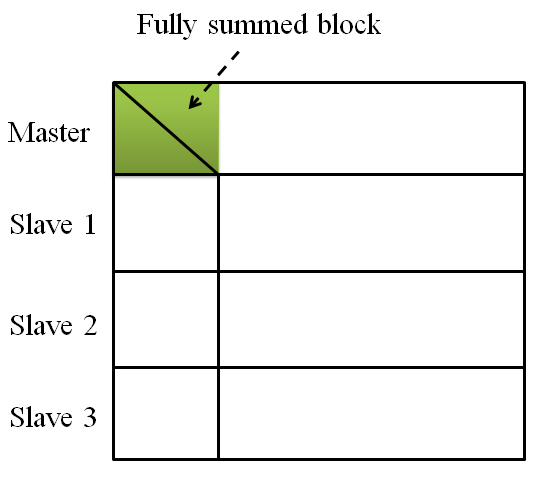
\includegraphics[width=0.45\textwidth]{figures/chapter-2/mumps-type-2-frontal-matrix.png}
\caption{MUMPS: static and dynamic scheduling}
\label{fig:mumps:type-2-frontal-matrix}
\end{figure}


\figpointer{fig:mumps:steps-of-type-2-factorization}
\begin{figure}[htpb]
  \centering
  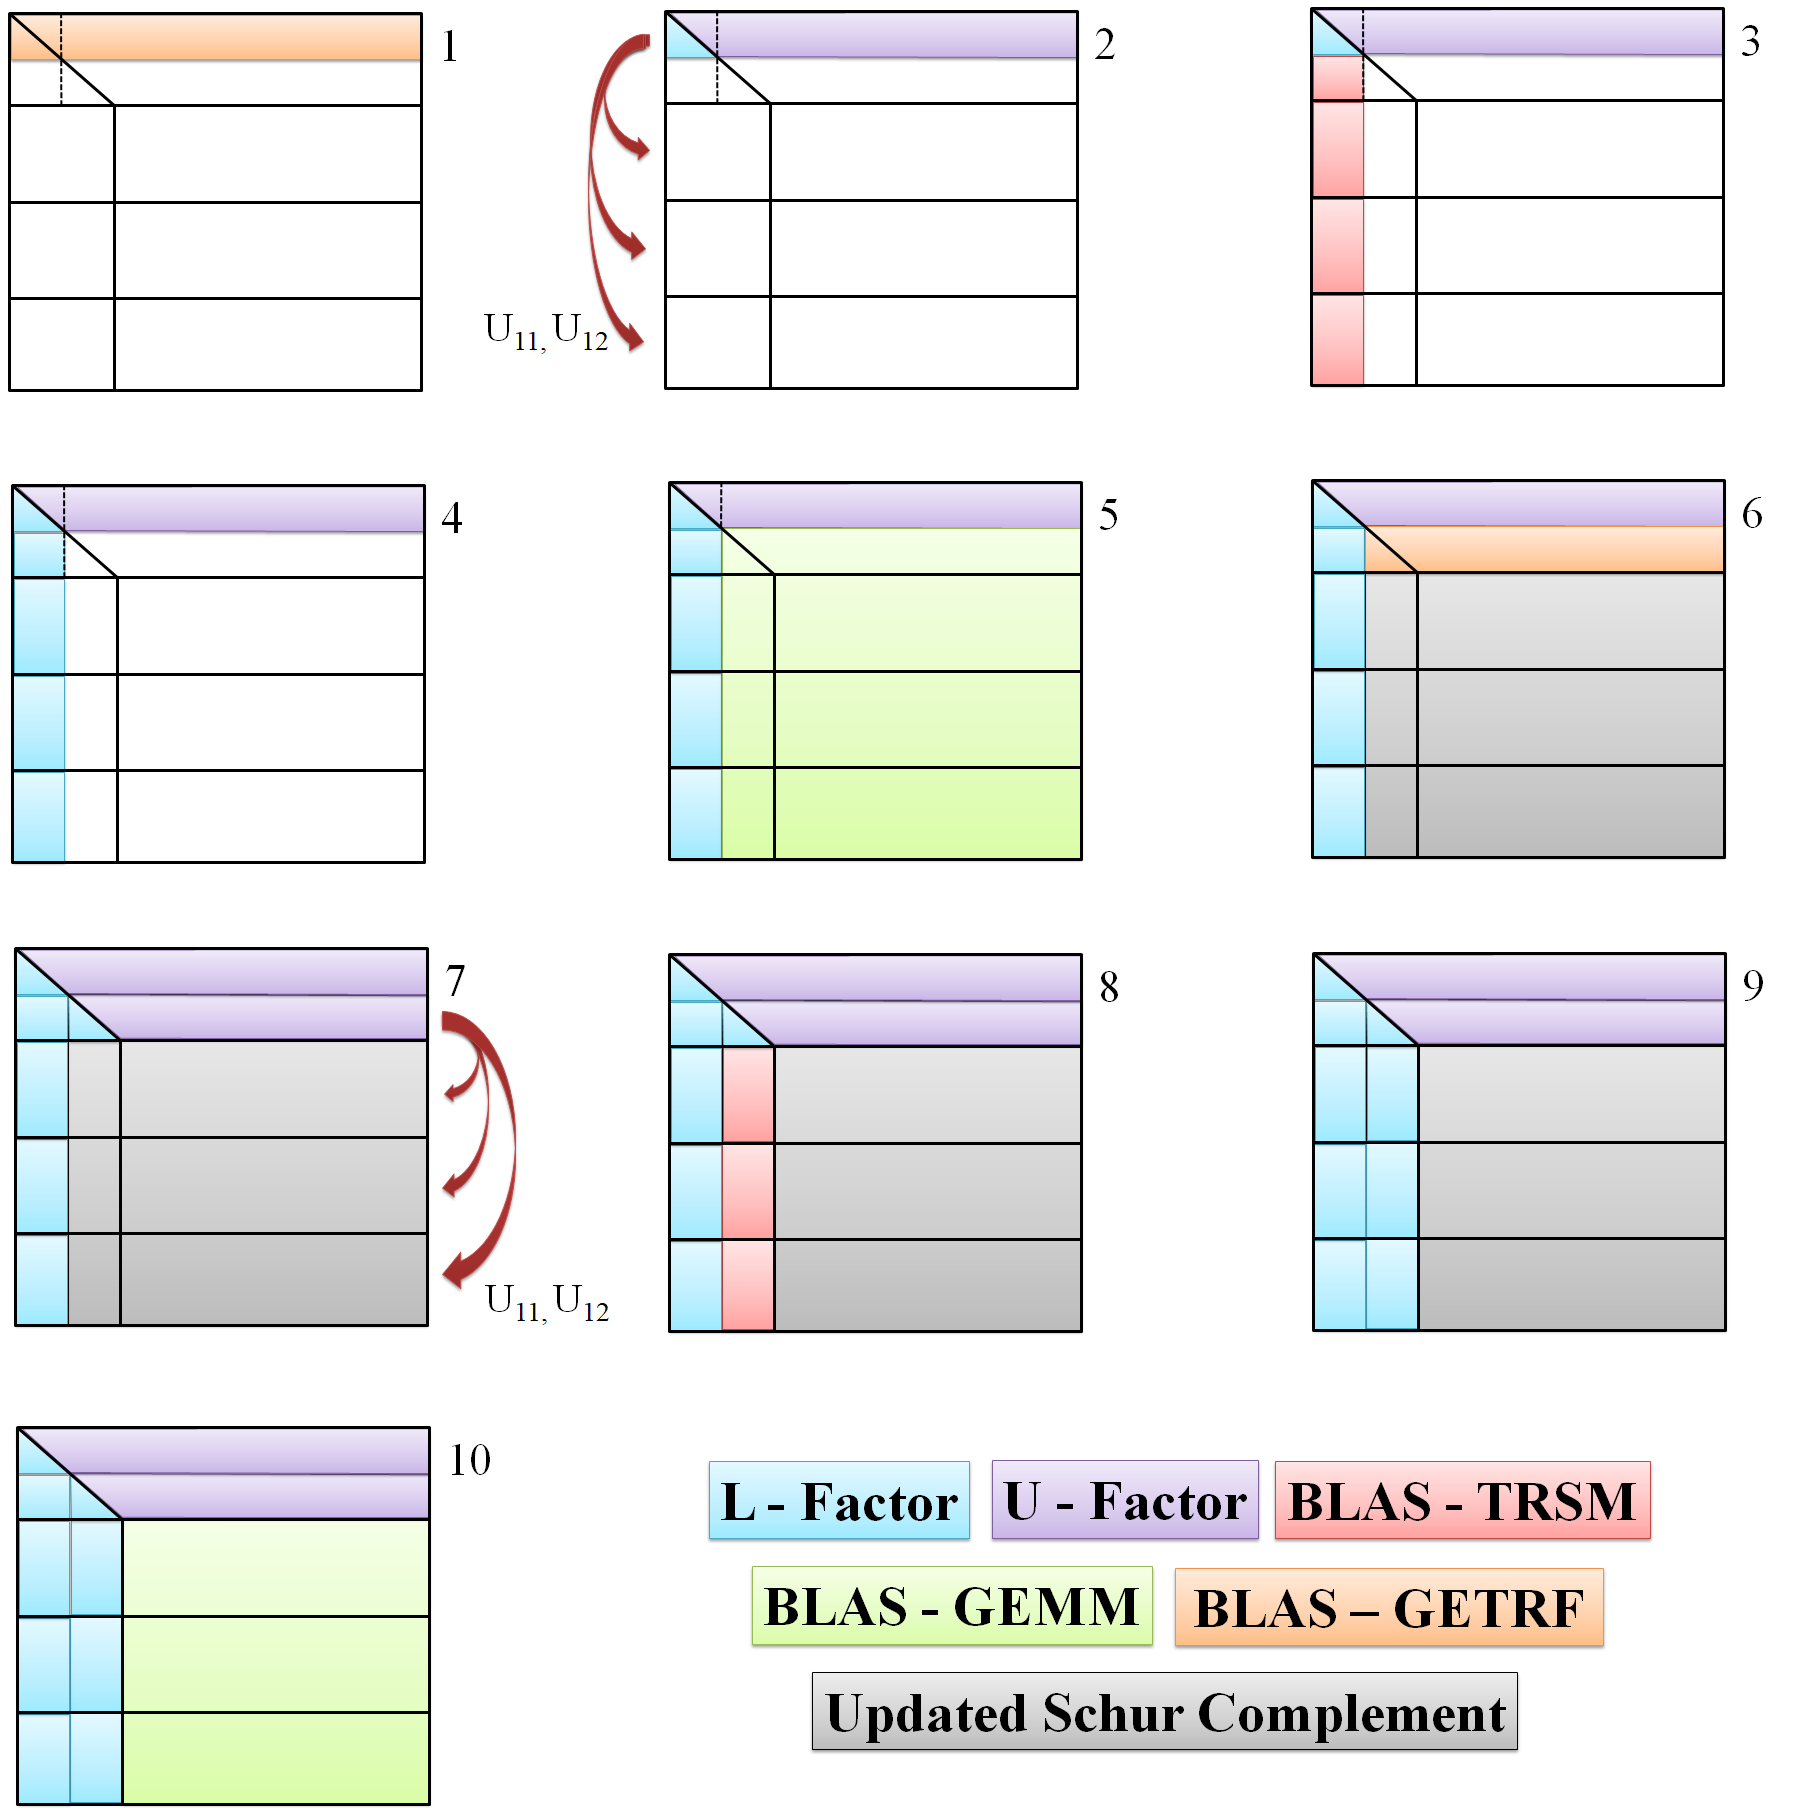
\includegraphics[width=0.85\textwidth]{figures/chapter-2/mumps-type-2-part-1.png}
\caption{MUMPS: An example of a type 2 node factorization}
\label{fig:mumps:steps-of-type-2-factorization}
\end{figure}


Both BLAS and LAPACK originate from the Netlib project which is a repository of numerous scientific computing software maintained by AT\&T Bell Laboratories, the University of Tennessee, Oak Ridge National Laboratory and other scintific communities \cite{netlib-overview}.\\


The goal of BLAS library is to provide a high efficient implementation of common dense linear algebra kernels by means of high rate of floating point operations per memory access, low cache and Translation Lookaside Buffer (TLB) miss rates.\\


In its turn, LAPACK is designed in such a way so that as much as possible of computation is performed by calls to BLAS library. This allows to achieve high efficiency for operations such as $LU$, $QR$, $SVD$ decompositions, triangular solve, etc. on modern computers. However, the Netlib BLAS implementation is written for an abstract general-purpose central processing unit, in mind, where hardware parameters are based on market statistics. Hence, it is not possible to achieve the maximum possible performance on a specific machine.\\


Hence, there exist special-purpose, hardware-specific implementations of the library developed by hardware vendors i.e. IBM, Cray, Intel, AMD, etc., as well as open-source tuned implementations such as ATLAS, OpenBLAS, etc. To achieve full compatibility, the developers consider the Netlib implementation of BLAS library as the standard (or reference) and thus overwrite all subroutines with additional tuning and optimization. This approach makes it possible to easily replace different BLAS implementations during object files linking  without any modifications of the source code.\\
 

Table \ref{table:list-of-blas-implementations} shows commercial and open-source tunned BLAS implementations available on the market today.\\

\begin{table}[h!]
\centering
\begin{tabular}{|c|c|c|}
\hline
Name                                                                 & Description                                                                                                                                                 & License                                                       \\ \hline
Accelerate                                                           & Apple's implementation for macOS and iOS                                                                                                                    & \begin{tabular}[c]{@{}c@{}}proprietary\\ license\end{tabular} \\ \hline
ACML                                                                 & BLAS implementation for AMD processors                                                                                                                      & \begin{tabular}[c]{@{}c@{}}proprietary\\ license\end{tabular} \\ \hline
C++ AMP                                                              & Microsoft's AMP language extension for Visual C++                                                                                                           & \begin{tabular}[c]{@{}c@{}}open\\ source\end{tabular}         \\ \hline
ATLAS                                                                & Automatically tuned BLAS implementation                                                                                                                     & \begin{tabular}[c]{@{}c@{}}open\\ source\end{tabular}         \\ \hline
Eigen BLAS                                                           & \begin{tabular}[c]{@{}c@{}}BLAS implemented on top of \\ the MPL-licensed Eigen library\end{tabular}                                                        & open source                                                   \\ \hline
ESSL                                                                 & optimized BLAS implementation for  IBM's machines                                                                                                           & \begin{tabular}[c]{@{}c@{}}proprietary\\ license\end{tabular} \\ \hline
GotoBLAS                                                             & Kazushige Goto's implementation of BLAS                                                                                                                     & \begin{tabular}[c]{@{}c@{}}proprietary\\ license\end{tabular} \\ \hline
HP MLIB                                                              & \begin{tabular}[c]{@{}c@{}}BLAS implementation supporting IA-64, PA-RISC, x86 \\ and Opteron architecture\end{tabular}                                      & \begin{tabular}[c]{@{}c@{}}proprietary\\ license\end{tabular} \\ \hline
Intel MKL                                                            & \begin{tabular}[c]{@{}c@{}}Intel's implementation of BLAS optimized for\\ Intel Pentium, Core,  Xeon and Xeon Phi\end{tabular}                              & \begin{tabular}[c]{@{}c@{}}proprietary\\ license\end{tabular} \\ \hline
Netlib BLAS                                                          & The official reference implementation on Netlib                                                                                                             & \begin{tabular}[c]{@{}c@{}}open\\ source\end{tabular}         \\ \hline
OpenBLAS                                                             & Optimized BLAS library based on GotoBLAS                                                                                                                    & \begin{tabular}[c]{@{}c@{}}open\\ source\end{tabular}         \\ \hline
PDLIB/SX                                                             & BLAS library targeted to the NEC SX-4 system                                                                                                                & \begin{tabular}[c]{@{}c@{}}proprietary\\ license\end{tabular} \\ \hline
SCSL                                                                 & BLAS implementations for SGI's Irix workstations                                                                                                            & \begin{tabular}[c]{@{}c@{}}proprietary\\ license\end{tabular} \\ \hline
\begin{tabular}[c]{@{}c@{}}Sun\\ Performance \\ Library\end{tabular} & \begin{tabular}[c]{@{}c@{}}Optimized BLAS and LAPACK for SPARC, Core \\ and AMD64 architectures under \\ Solaris 8, 9, and 10 as well as Linux\end{tabular} & \begin{tabular}[c]{@{}c@{}}proprietary\\ license\end{tabular} \\ \hline
\end{tabular}
\caption{Comerrcial and open source BLAS implementations \cite{wiki:blas-implementations}}
\label{table:list-of-blas-implementations}
\end{table}



Among all libraries listed in table \ref{table:list-of-blas-implementations} there were only four available on HW1 machine, namely: Netlib BLAS, Intel MKL, OpenBLAS and ATLAS. However, installation of ATLAS requires to switch off dynamic frequency scaling, also called CPU throttling, to allow an ATLAS configuration routine to find the best loop transformation parameters for a specific hardware. In order to turn off CPU throttling, one has to reboot the entire machine and make appropriate changes in Basic Input/Output System (BIOS). This fact made ATLAS library not to be suitable for the rest of the research and we excluded it from our primary list of candidates. Moreover, during installation, one has to explicitly provide the number of OpenMP threads that are going to be used once a BLAS subroutine is called. This means there is no way to change the number of threads per MPI process in run-time without re-installation of ATALS library. Thus, only 3 versions of MUMPS-PETSc (Netlib BLAS, Intel MKL and OpenBLAS) libraries were compiled and tested with using GRS matrix set and 1 thread per MPI process. The test results are shown in figures bla, bla and bra.\\



% say that ATLAS is shit and we have to live only with Intel MKL and OpenBlas

% Say that we are going to use Netlib blas as the baseline